%=================================================================
% RiskPredictor: a risk engine for sports prediction markets
% Built on Prof. Shasha's MDPI Forecasting template (Definitions/mdpi.cls).
% Compile: pdflatex riskpredictor; bibtex riskpredictor; pdflatex riskpredictor; pdflatex riskpredictor
%=================================================================
\documentclass[forecasting,article,accept,pdftex,moreauthors]{Definitions/mdpi}

\usepackage{verbatim}
\usepackage{makecell}
\usepackage{subcaption}
\usepackage{graphicx}
\usepackage{float}
\usepackage{booktabs}
\usepackage{listings}
\usepackage{comment}
\usepackage{enumitem}
\graphicspath{{figures/}}
\newcommand{\aname}{{{\it RiskPredictor}}}

%=================================================================
% MDPI internal commands - do not modify
\firstpage{1}
\makeatletter
\setcounter{page}{\@firstpage}
\makeatother
\pubvolume{1}
\issuenum{1}
\articlenumber{0}
\pubyear{2026}
\copyrightyear{2026}
\externaleditor{Academic Editor(s): Name}
\datereceived{ }
\daterevised{ }
\dateaccepted{ }
\datepublished{ }
\hreflink{https://doi.org/}

%=================================================================
\Title{\aname: Pricing and Risk for Sports Prediction Markets}
\TitleCitation{\aname: Pricing and Risk for Sports Prediction Markets}

\newcommand{\orcidauthorA}{0000-0002-7036-3312}

\Author{Sai Kishore Pathakamuri $^{1,\dagger}$ and Dennis Shasha $^{2,}$*\orcidA{}}
\AuthorNames{Sai Kishore Pathakamuri and Dennis Shasha}
\AuthorCitation{Pathakamuri, S.K.; Shasha, D.}

\address{%
$^{1}$ \quad Department of Finance and Risk Engineering, NYU Tandon School of Engineering, 6 MetroTech Center, Brooklyn, NY 11201 USA; sp8744@nyu.edu\\
$^{2}$ \quad Courant Institute of Mathematical Sciences, 251 Mercer Street, New York, NY 10012 USA; des1@nyu.edu}

\corres{Correspondence: des1@nyu.edu}

\abstract{Prediction markets on sporting events now trade billions of contracts a season, yet the risk tools of traditional finance assume continuous prices and long histories that binary, short-lived contracts do not have. We set out to build a risk engine for such markets and argue that its core is a probability model of game outcomes: a contract's price is a probability, so pricing and settlement risk are the same calculation, and a joint model over the final score prices every contract on a game consistently and lets risk net across them. We survey the literature on predicting NFL games, build a leak-free table of 759 pre-game features for 7,548 games (1999--2026), and fit a two-output random forest that predicts both teams' scores. Evaluated walk-forward over sixteen seasons, it predicts the margin with a mean absolute error of 10.35 points against 10.38 for Elo and 10.05 for the Vegas closing line, matching the published literature. Its score predictions are calibrated, its residuals are uncorrelated with standard deviations of 9.6 and 9.4 points, and, placed on an empirical score grid that preserves the NFL's key-number spikes, they price the full ladder of spread and total contracts to within a cent of the Kalshi order book. Ensembles with public forecasts do not beat the closing line. We conclude that the engine's value lies in a calibrated joint distribution rather than a better point forecast, and set out the next steps.}

\keyword{prediction markets; sports betting; risk management; random forests; expected shortfall; Kalshi; NFL; score prediction}

\begin{document}

\section{Introduction}

Prediction markets have moved from a niche into the mainstream. On Kalshi alone the three main contract types on a single NFL week (game winner, point spread, game total) traded close to two billion contracts over the first three weeks of the 2026 season, and the Super Bowl winner market carries over a hundred million contracts of open interest. In this document we explore how the methods of traditional financial risk management apply to such markets and build a risk engine for them, \aname.

The goals of the engine are:
\begin{enumerate}[nosep]
\item compute security-level and portfolio-level risk;
\item in computing portfolio risk, add or net exposures according to the defined behaviour of the assets (netting through correlation, or, as we argue below, through a joint outcome model);
\item produce metrics that show what a book would actually do when the market moves;
\item at a later stage, support margin, collateral and leverage calculations;
\item identify cross-market hedging opportunities that allow more balanced products and portfolios.
\end{enumerate}

\subsection{Contributions so far}

This document is a research record: each weekly report adds a section, and earlier sections are revised as the project develops. The contributions to date are:
\begin{enumerate}[nosep]
\item a classification of traditional risk tools into those that carry over to binary contracts unchanged, those that need adapting, and those that do not apply (Section~\ref{sec:tools});
\item the observation, developed in Section~\ref{sec:pricing}, that for a binary contract the price is the outcome probability and therefore the full profit-and-loss distribution, so a pricing model and a settlement-risk model are the same object, and that a joint model over the final score is what allows netting across contracts on the same game;
\item an empirical score distribution for NFL games that preserves the discrete structure of football scoring and prices every Kalshi contract on a game to within a cent of the live order book (Section~\ref{sec:pricing});
\item a literature survey of NFL score prediction and market efficiency (Section~\ref{sec:literature});
\item a leak-free pre-game feature table of 7,548 games and 805 columns, with a perturbation test for leakage (Section~\ref{sec:data});
\item a two-output random forest predicting both teams' scores, evaluated walk-forward over sixteen seasons against Elo and the closing line, with its residual structure, an ensemble test against public forecasts, and full outcome distributions compared with the Vegas lines (Section~\ref{sec:scoremodel}).
\end{enumerate}

\section{Risk Tools from Traditional Finance}\label{sec:tools}

Traditional risk tools were built for instruments whose prices move continuously and have long histories. Sports prediction contracts pay exactly \$1 or \$0, last hours or days, and move in jumps. As a result the \emph{processes} of traditional risk management carry over, the \emph{measures} need adapting, and the \emph{statistical assumptions} no longer hold. Table~\ref{tab:tools} summarises our classification.

\begin{table}[H]
\centering
\small
\begin{tabular}{p{2.6cm}p{5.2cm}p{6.2cm}}
\toprule
\textbf{Category} & \textbf{Tools} & \textbf{Why} \\
\midrule
Works as-is & Expected shortfall, scenario revaluation, SPAN margining, stress testing, limit frameworks, counterparty exposure & They work for any payoff shape. Because every possible outcome can be listed, they can be computed exactly. \\
Needs adapting & Greeks, jump-to-default, basket correlation, netting, liquidity-adjusted risk, backtesting & The concepts are valid but must be reworked for binary, jump-driven payoffs, where dependence between contracts comes mostly from their structure rather than from statistics. \\
Does not work & VaR as usually computed, covariance matrices, factor models, historical price simulation, continuous hedging & They assume smooth, normally distributed returns with long price histories, none of which exist here. \\
New to prediction markets & Resolution-rule risk, cross-venue basis risk, integrity risk & These have no direct equivalent in traditional finance. \\
\bottomrule
\end{tabular}
\caption{Traditional risk tools and how they transfer to binary sports contracts.}
\label{tab:tools}
\end{table}

\subsection{Terms}

\begin{description}[nosep,leftmargin=0pt,labelindent=0pt]
\item[Value at Risk (VaR)] the loss that will not be exceeded at a given confidence level (e.g.\ 95\%). It ignores how large losses can be beyond that point.
\item[Expected shortfall (ES)] the average loss in the worst outcomes beyond the VaR threshold, which captures the size of the tail.
\item[Scenario revaluation] repricing every position under each possible scenario and adding up the profit and loss.
\item[SPAN margining] setting collateral equal to the worst portfolio loss across a defined set of scenarios.
\item[Stress testing] measuring losses under extreme but plausible events. \emph{Reverse} stress testing finds the events that would cause a given loss.
\item[Greeks] sensitivities of a position's value. \emph{Delta} measures the response to price, \emph{gamma} how delta itself changes, and \emph{theta} the effect of time passing.
\item[Basket correlation] risk in a product that depends on several events together (e.g.\ a parlay), driven by how those events are related.
\item[Netting] offsetting gains and losses across related positions to find the true combined exposure.
\item[Liquidity-adjusted risk] risk measured at the price one could actually exit at, rather than the mid-price.
\item[Covariance matrix, factor model] statistical tools that estimate how assets move together from historical returns.
\item[Counterparty exposure] potential loss if a counterparty or venue fails to pay.
\item[Resolution-rule risk] loss from how a contract settles, e.g.\ voids, pushes, overtime or stat corrections.
\item[Cross-venue basis risk] the ``same'' contract settling differently on two platforms.
\item[Integrity risk] loss from insider information or match-fixing.
\end{description}

\subsection{Value at Risk}

VaR answers one question: how much could I lose over a given period, at a given confidence level, under normal market conditions? Every VaR number has three parts: a loss amount, a time horizon and a confidence level. It is traditionally computed in one of three ways: parametrically, assuming a normal distribution of the underlying; by historical simulation; or by Monte Carlo. Its limitations are well known. It says nothing about the size of losses beyond the threshold, so two portfolios can have the same VaR while one loses ten times more in the worst 1\% of cases. It is not subadditive, so VaR$(A+B)$ can exceed VaR$(A)$ + VaR$(B)$, which makes diversification appear to increase risk; for this reason it is not a coherent risk measure in the sense of Artzner et al.~\cite{artzner1999}. And it relies on normal conditions, while correlations and volatilities shift sharply in a crisis.

\subsection{VaR and expected shortfall for binary contracts}\label{sec:binaryvar}

For a binary contract none of the three traditional computations is needed, because the loss distribution can be written down. A position of $q$ contracts bought at price $p$ pays $q(1-p)$ if the event occurs and loses $qp$ otherwise. If the true probability of the event is $\pi$, the profit-and-loss distribution has exactly two points. At confidence level $\alpha$,
\[
\mathrm{VaR}_\alpha = \begin{cases} qp & \text{if } 1-\pi > 1-\alpha,\\ 0 & \text{otherwise,}\end{cases}
\qquad
\mathrm{ES}_\alpha = \frac{qp\,\min(1-\pi,\,1-\alpha)}{1-\alpha}.
\]
So for a single contract the whole of risk measurement reduces to one number, $\pi$, which is also the fair price. For a portfolio of contracts on the same game the loss distribution is a sum over the joint outcomes of the game: with a probability table $p(h,a)$ over the final score, each position's payoff is a function of $(h,a)$, the portfolio profit and loss is their sum cell by cell, and VaR, ES, the worst case and the probability of loss are read directly from the resulting distribution with no simulation and no covariance matrix. This is the sense in which the pricing model and the risk model are the same object, and it is why the rest of this document is about building $p(h,a)$.

\section{Data}\label{sec:data}

\subsection{Kalshi}

Kalshi is a regulated US exchange on which event contracts trade in a central limit order book, each contract paying \$1 if the event occurs. Table~\ref{tab:kalshi_series} lists the NFL contract series with their volume at the time of our first survey. Game-level contracts (winner, spread, total) are the focus of this project because they are the ones a joint score model prices directly.

\begin{table}[H]
\centering
\small
\begin{tabular}{llrrr}
\toprule
\textbf{Series} & \textbf{Type} & \textbf{Open markets} & \textbf{Volume (contracts)} & \textbf{Open interest} \\
\midrule
KXSB & Super Bowl winner & 32 & 131.9M & 108.0M \\
KXNEXTTEAMNFL & Player next team & 290 & 4.69M & 2.86M \\
KXNFLGAME & Game winner (moneyline) & 64 & 4.60M & 3.93M \\
KXNFLDPOTY & Defensive player of the year & 65 & 2.32M & 2.13M \\
KXNFLPLAYOFF & Playoff qualifiers & 32 & 1.85M & 1.20M \\
KXNFLNFCEAST & Division winner & 4 & 1.59M & 1.17M \\
KXNFLSPREAD & Point spread & 414 & 1.40M & 1.22M \\
KXNFLTOTAL & Game total & 304 & 1.16M & 1.12M \\
KXNFLAFCNORTH & Division winner & 4 & 0.79M & 0.64M \\
KXNFL1SEED & Conference 1 seed & 32 & 0.64M & 0.56M \\
KXNFLFFLEADER & Fantasy positional leader & 361 & 0.47M & 0.41M \\
KXLEADERNFLPYDS & Passing yards leader & 28 & 0.28M & 0.26M \\
KXNFLRECYDS & Receiving yards prop & 437 & 0.19M & 0.18M \\
KXNFLRSHYDS & Rushing yards prop & 289 & 0.13M & 0.13M \\
\bottomrule
\end{tabular}
\caption{Kalshi NFL contract series, September 2026 snapshot of open markets.}
\label{tab:kalshi_series}
\end{table}

We pulled, through the Kalshi REST API, every market in the winner, spread and total series listed since May 2026 (5,402 markets on 354 events), their complete trade tape (12.9 million trades, 1.98 billion contracts), and hourly candlesticks with best bid and ask, volume and open interest (1.17 million candles). The 2025 season is archived out of the public API. Three facts from this data shape the design: 82\% of winner-contract volume trades after kickoff; the book sits at the 1-cent minimum tick for nearly all of game day, so the mid-price is a clean quote; and hourly price changes have a standard deviation of about 17 cents in play against 1 cent before the game, so in-play risk is inventory risk rather than liquidity risk. Spread strikes are listed every half point from $\pm1.5$ to about $\pm30$ for each team, and totals every half point over roughly $\pm20$ points around the line, so a game's ladder pins the market-implied distribution of margin and total at some 45 points. Pre-kickoff prices are well calibrated (Figure~\ref{fig:kalshi_cal}) and within 1.1 percentage points of the de-vigged sportsbook closing line on average.

\begin{figure}[H]
\centering
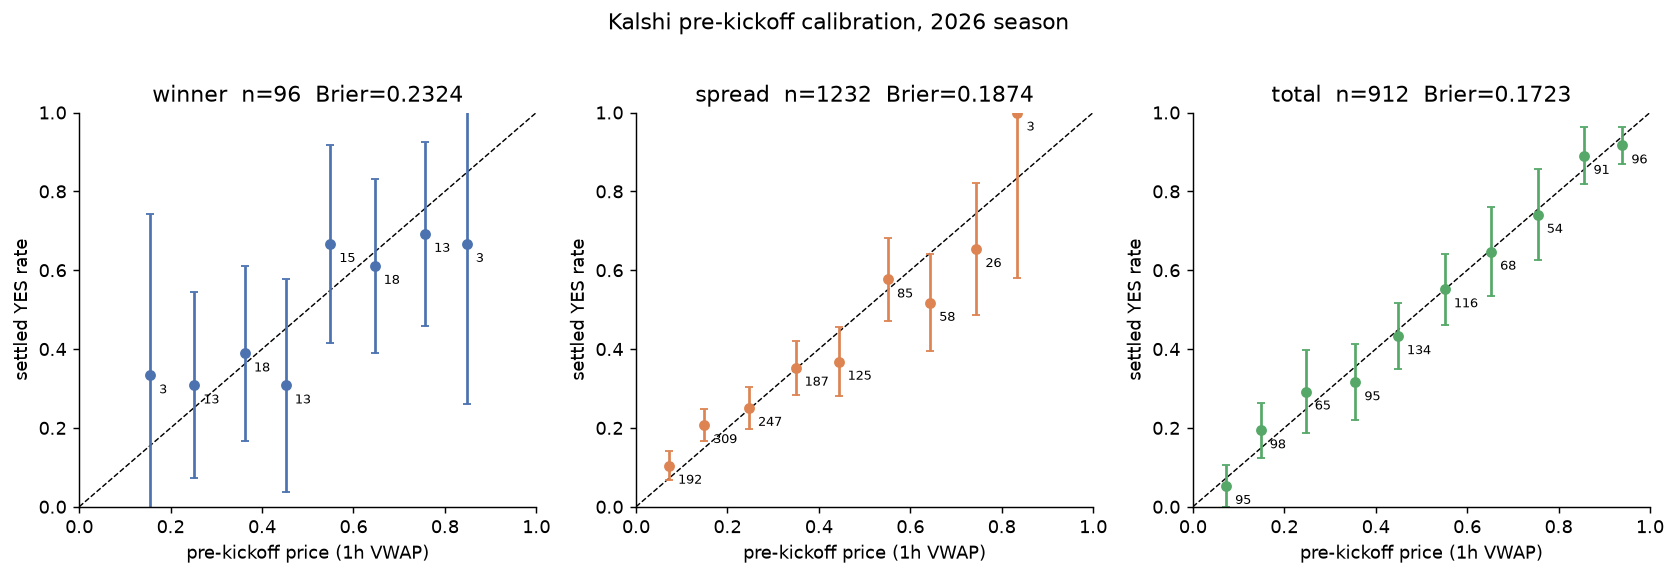
\includegraphics[width=0.95\textwidth]{kalshi_calibration.png}
\caption{Calibration of Kalshi pre-kickoff prices (1-hour volume-weighted average) against settlement, 2026 weeks 1--3, by contract type.}
\label{fig:kalshi_cal}
\end{figure}

\subsection{NFL results and the pre-game feature table}

Historical results, play-by-play, rosters, injury reports and closing lines come from the public nflverse project~\cite{nflverse}. From them we built a table of 7,548 games (1999--2026) with 805 columns, one row per game in home-team orientation (Table~\ref{tab:features}). All data is free.

\begin{table}[H]
\centering
\small
\begin{tabular}{p{2.2cm}rp{8.3cm}p{1.9cm}}
\toprule
\textbf{Group} & \textbf{Cols} & \textbf{Content} & \textbf{From} \\
\midrule
Team form & 604 & 20 offensive and 20 defensive efficiency statistics from play-by-play (EPA per play, success rate, pass and rush splits, explosive-play rate, yards per play, completion percentage over expected, turnovers, sacks, third-down rate, points per drive, neutral-script EPA), each over five windows (last 4, last 8, exponentially weighted, season to date, previous season), for home, away and the home-minus-away difference & 1999; CPOE 2006 \\
Ratings & 68 & Pre-game Elo (FiveThirtyEight recipe), exponentially weighted margin, opponent-adjusted margin & 1999 \\
Quarterback & 23 & Scheduled starter's weighted EPA per dropback, CPOE, sack and interception rates, career dropbacks, starter-change flag & 1999 \\
Injuries & 44 & Players Out/Doubtful and Questionable by position group; snap share of players now out & 2009; snaps 2013 \\
Situational & 31 & Rest, bye, short week, primetime, dome, surface, temperature, wind, divisional, playoff & 1999 \\
Market & 10 & Closing spread, total, moneylines; stored for benchmarking, never used as features & 1999 \\
Targets & 5 & Home score, away score, margin, total, home win & 1999 \\
\bottomrule
\end{tabular}
\caption{The pre-game feature table.}
\label{tab:features}
\end{table}

Every feature is computed from information dated before kickoff: rolling statistics are shifted by one game, Elo is the pre-update value, and injury counts come from the report filed before the game. Following Glickman and Stern~\cite{glickmanstern2017}, each team statistic enters as the home value, the away value and their difference. We test for leakage by perturbation: one game's play-level statistics are multiplied by ten and thirty points added to its score, the table is rebuilt, and the game's own 233 team features and Elo must be unchanged while the two teams' later games change. Six random games pass. The test earned its keep: the nflverse schedule carries two post-game fields, \texttt{result} and \texttt{total}, that equal the targets. A forest trained with them reported a margin error of 2.4 points with 85\% of its importance on those two columns; they were removed and the table re-scanned for any column correlated above 0.6 with a target.

\subsection{Testing}

All programs are implemented in Python in a shared repository and run locally or on Google Colab. Models are evaluated walk-forward by season, training on all seasons before $t$ and testing on season $t$, because games within a season are related through the teams.

\section{Pricing a Contract Is Modelling the Outcome}\label{sec:pricing}

\subsection{Price, probability and settlement risk}

A binary contract's price is, up to the exchange's fee and spread, the market's probability of the outcome. With only two outcomes, that probability \emph{is} the full profit-and-loss distribution (Section~\ref{sec:binaryvar}). Pricing and settlement risk are therefore the same calculation. For a portfolio, the pricing model must be a joint one, because the joint probabilities are what allow risk to net across positions.

A proper joint outcome model, such as a distribution over the final score of a game, gives everything in Table~\ref{tab:joint_uses} at once.

\begin{table}[H]
\centering
\small
\begin{tabular}{p{6.5cm}p{6.5cm}}
\toprule
\textbf{Output} & \textbf{Used for} \\
\midrule
Fair price of every contract on the game & Pricing \\
Probability of each outcome state & ES, probability of loss, expected loss \\
Joint behaviour of contracts on the same game & Netting (goal 2 of the engine) \\
Consistent prices across winner, spread, total and props & Detecting mispricing between related contracts \\
\bottomrule
\end{tabular}
\caption{What a joint outcome model provides.}
\label{tab:joint_uses}
\end{table}

Every Kalshi contract on a game is a region of the final-score grid. With $h$ and $a$ the home and away scores, the winner contract pays when $h-a>0$ (ties settle at \$0.50), a spread contract at strike $k$ pays when $h-a>k$, and a total contract pays when $h+a>k$. One probability table $p(h,a)$ prices all of them by summing cells, and a book of positions is a payoff vector over the same grid.

\subsection{What the empirical score distribution looks like}

Three findings from 3,076 games (2015--2026) constrain the shape of $p(h,a)$ (Figure~\ref{fig:keynumbers}). The absolute margin lands exactly on 3 in 14.8\% of games and on 7 in 8.7\%, 2.9 and 1.9 times what a normal distribution centred on the point spread implies; a smooth model misprices spread strikes near these ``key numbers'' by 5 to 10 cents. Margin and total are nearly uncorrelated (0.03) but share parity in every game, since they are the difference and sum of the same two integers, so half of the margin-by-total lattice is empty and a copula on the two marginals would put mass there. And the closing spread is an unbiased forecast with a residual standard deviation of 12.7 points, slightly tighter than the 13.86 of Stern~\cite{stern1991}.

\begin{figure}[H]
\centering
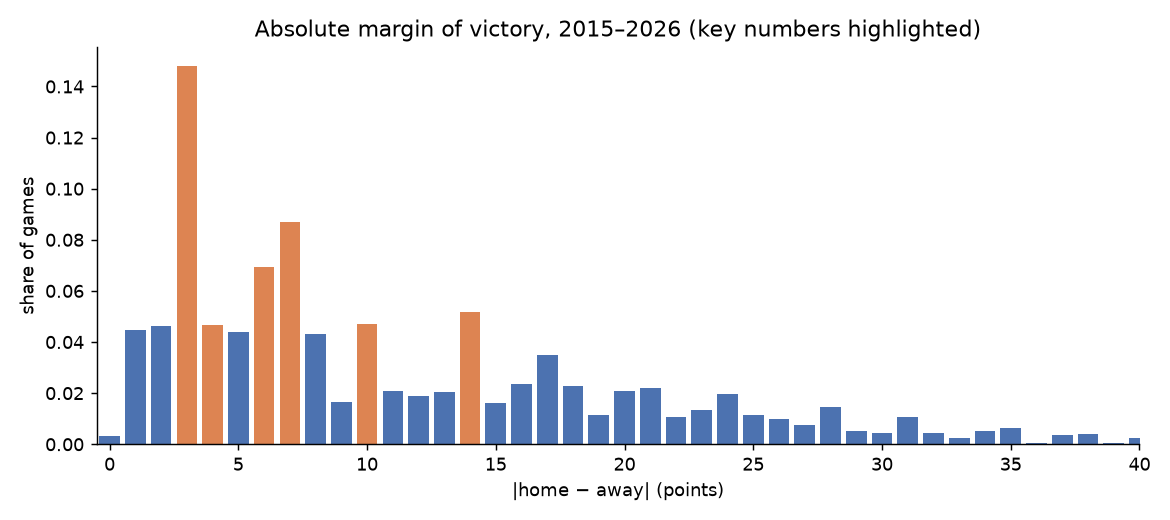
\includegraphics[width=0.95\textwidth]{nfl_abs_margin.png}
\caption{Absolute margin of victory, 2015--2026 (3,076 games); key numbers 3, 7, 6, 10 and 14 in orange.}
\label{fig:keynumbers}
\end{figure}

\begin{figure}[H]
\centering
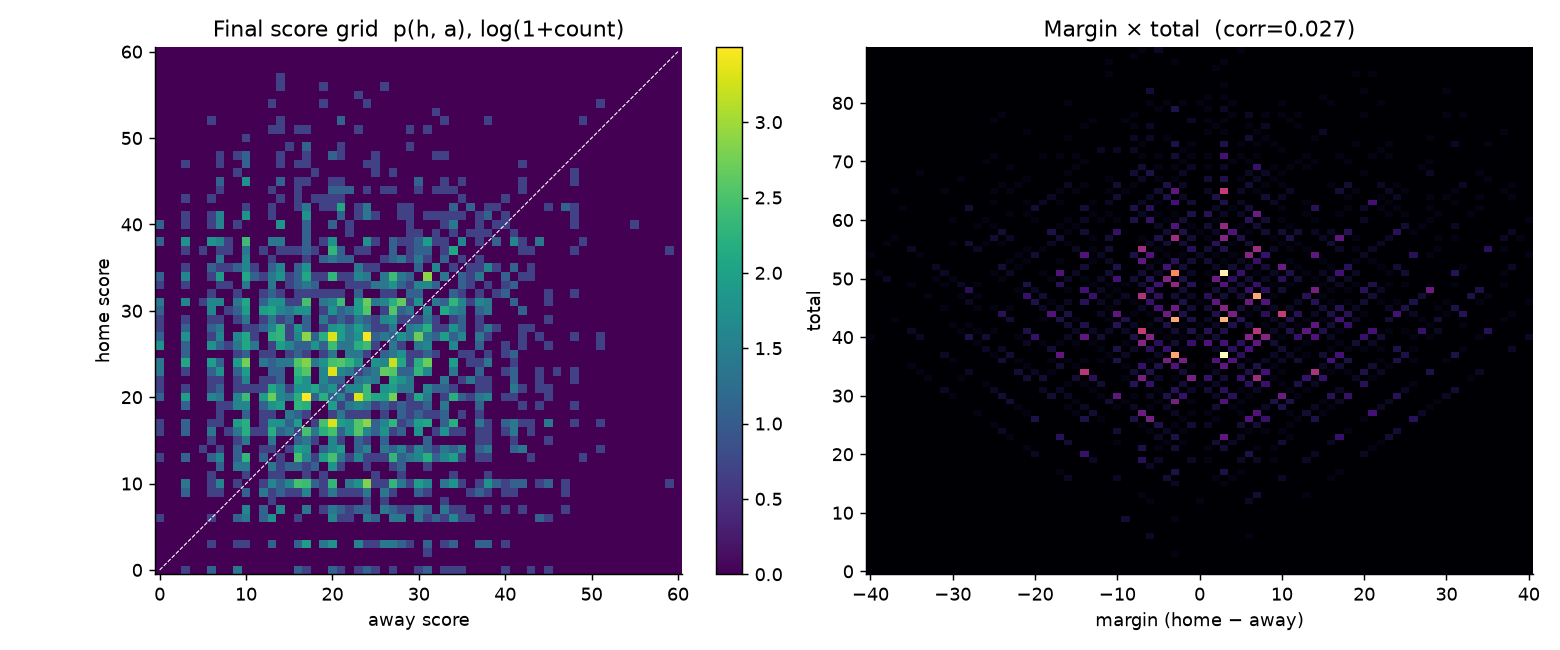
\includegraphics[width=0.95\textwidth]{nfl_score_grid.png}
\caption{Left: the empirical final-score grid $p(h,a)$ (log counts). Right: margin against total; the chequerboard is parity.}
\label{fig:scoregrid}
\end{figure}

\subsection{Positioning the empirical distribution for a game}

We want a distribution $p$ that (i) has the game's expected margin and total and (ii) is otherwise as close as possible to the historical prior $p_0$. Minimising the Kullback--Leibler divergence $\mathrm{KL}(p\,\|\,p_0)$ subject to the two moment constraints gives the exponential-family solution
\begin{equation}
p(h,a) \;\propto\; p_0(h,a)\,\exp\!\big(\lambda_1 (h-a) + \lambda_2 (h+a)\big),
\label{eq:tilt}
\end{equation}
with $(\lambda_1,\lambda_2)$ solved so that $\mathbb{E}[h-a]$ and $\mathbb{E}[h+a]$ match the targets, a two-equation root find. Because the tilt only reweights cells, it cannot create mass where the prior has none: a 3-point win stays 2.9 times as likely as a 4-point win. A Poisson or normal model would have to be taught key numbers, parity and cell clustering; the empirical grid already has them.

\paragraph{Worked example.} Pittsburgh at Cleveland, 1 October 2026, with the live Kalshi order book captured the day before (46 contracts). The sportsbook line was Cleveland $-2.5$ and total 38.5. Tilting the 3,076-game prior to those two numbers gives $\lambda_1=-0.0222$, $\lambda_2=-0.0399$ (Figures~\ref{fig:toy_dist} and~\ref{fig:toy_grid}). Table~\ref{tab:toy} compares model prices with the Kalshi mid for every contract.

\begin{figure}[H]
\centering
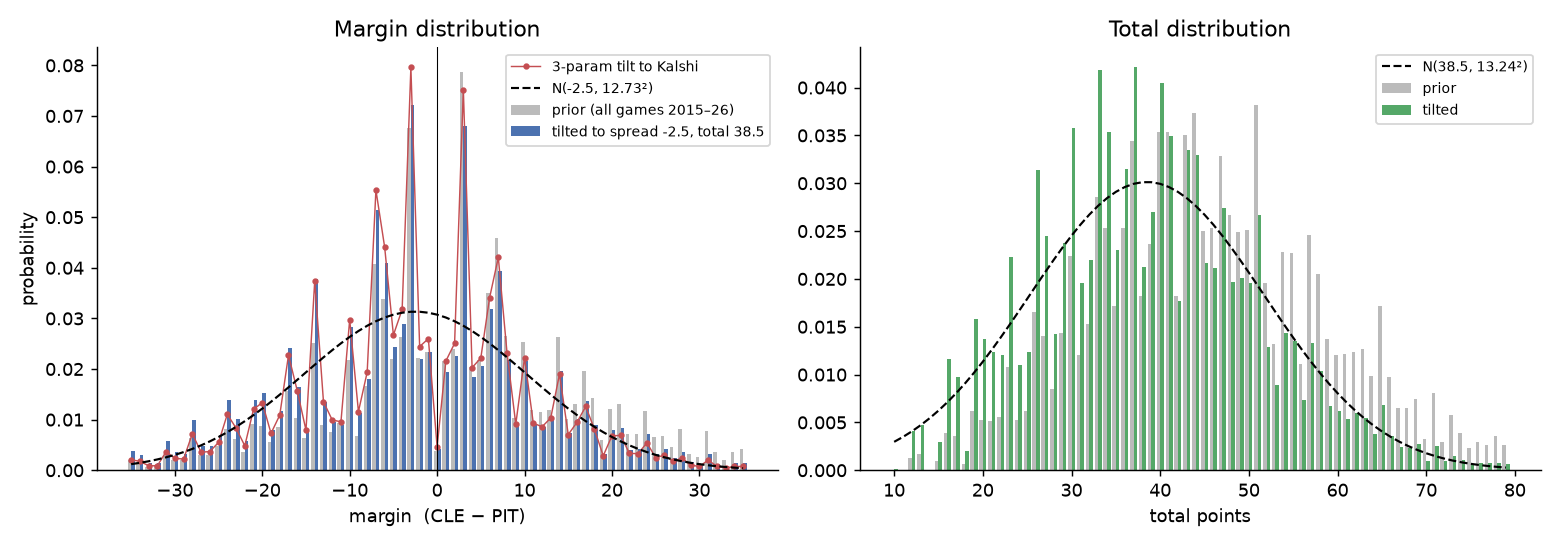
\includegraphics[width=0.98\textwidth]{toy_margin_total.png}
\caption{Margin (left) and total (right) distributions: grey the prior, blue the prior tilted to the book line, red a three-parameter tilt calibrated to Kalshi, dashed the normal.}
\label{fig:toy_dist}
\end{figure}

\begin{figure}[H]
\centering
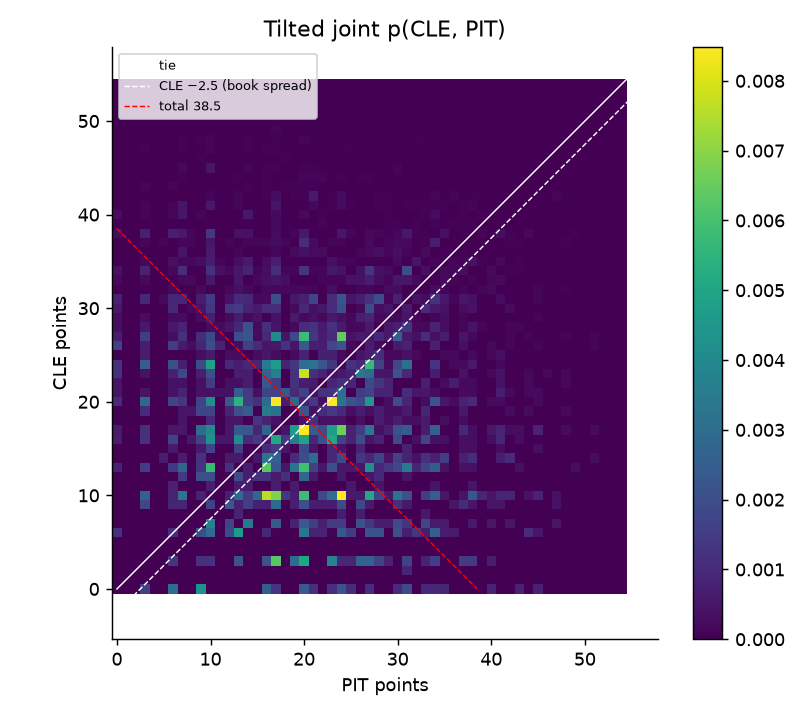
\includegraphics[width=0.6\textwidth]{toy_joint_grid.png}
\caption{The tilted joint table for Pittsburgh at Cleveland. The diagonal is a tie, the dashed line the book spread and the red line the total; each contract is a sum over one side of one of these lines.}
\label{fig:toy_grid}
\end{figure}

\begin{table}[H]
\centering
\small
\begin{tabular}{lcccc}
\toprule
\textbf{Model} & \textbf{All 46} & \textbf{Winner} & \textbf{Spread strikes} & \textbf{Total strikes} \\
\midrule
Untilted prior & 11.2 & 12.5 & 8.7 & 14.3 \\
Normal around the line & 1.89 & 0.28 & 2.32 & 1.48 \\
Tilt to the book line (no Kalshi data) & 1.52 & 0.08 & 1.98 & 1.06 \\
Two-parameter tilt fitted to Kalshi mids & 1.49 & 0.76 & 2.00 & 0.88 \\
Three-parameter tilt (adds margin$^2$) fitted to Kalshi & 0.76 & 0.24 & 0.64 & 0.99 \\
\bottomrule
\end{tabular}
\caption{Mean absolute error in cents of model price against the Kalshi mid, Pittsburgh at Cleveland. Quoted bid--ask spreads were 1--2 cents.}
\label{tab:toy}
\end{table}

\begin{figure}[H]
\centering
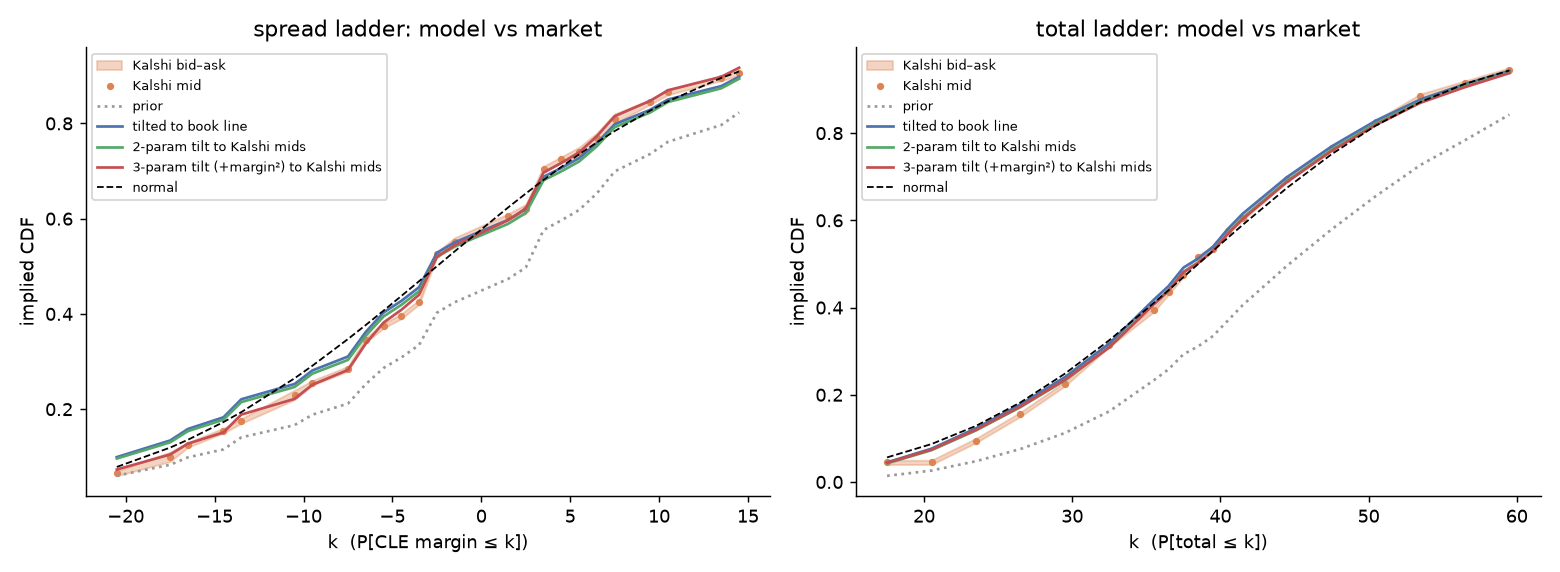
\includegraphics[width=0.98\textwidth]{toy_ladders.png}
\caption{Market-implied cumulative distributions from the spread (left) and total (right) ladders against the model variants. The shaded band is the Kalshi bid--ask.}
\label{fig:toy_ladders}
\end{figure}

Three lessons follow. Locating the distribution with the book line removes 87\% of the pricing error and prices the winner contract to 0.1 cents. Discreteness matters on the ladder: the normal is off by up to 6 cents on a single strike. And two moments do not control the tails: the book-tilted grid overprices Pittsburgh blowouts by 2--4.5 cents because the prior's margin has standard deviation 14.2 while the market prices this low-scoring game nearer 12.3. A third parameter on $(h-a)^2$ lets the market set the dispersion and the tail error disappears. This is the strongest argument for a model that predicts dispersion as well as location, and it motivates the score model of Section~\ref{sec:scoremodel}.

\subsection{What moves a game's expected score}

Before building features we listed the factors practitioners weigh when setting a line (Table~\ref{tab:factors}); the feature table of Section~\ref{sec:data} covers all but travel distance.

\begin{table}[H]
\centering
\small
\begin{tabular}{p{3cm}p{2.4cm}p{8.4cm}}
\toprule
\textbf{Factor} & \textbf{Typical effect} & \textbf{Notes} \\
\midrule
Starting quarterback & $\pm$3 to 10 pts & The largest single factor; elite starter versus backup is worth 7--10 points or 20--25 percentage points of win probability. Status should be modelled as a probability when questionable. \\
Team strength & baseline & Elo or power ratings, or EPA per play and success rate on offence and defence; adjust for opponent and regress toward the mean early in the season. \\
Home field & 1.5 to 2 pts & Has shrunk over the past decade; varies by venue and travel. \\
Other key injuries & 0.5 to 2 pts each & Costliest at offensive tackle, edge rusher, top cornerback and top receiver; multiple injuries on one unit compound. \\
Rest and schedule & 0.5 to 1.5 pts & Bye week helps; short week and long road trips hurt; time-zone changes matter for early-kickoff West Coast teams. \\
Weather and venue & totals & Wind above 15 mph and heavy precipitation suppress scoring; lowers the total and compresses variance. Domes remove it. \\
Coaching & 0.5 to 1 pt & Fourth-down aggressiveness, clock management, in-game adjustments. \\
Motivation and context & small, noisy & Playoff seeding, eliminated teams and week-18 rest can matter in specific spots. \\
Turnover luck & shrinkage & Fumble recoveries and close-game records are largely noise; use them to shrink apparent strength. \\
\bottomrule
\end{tabular}
\caption{Factors in a game's expected score, with typical magnitudes as cited by practitioners.}
\label{tab:factors}
\end{table}

\section{Literature: Predicting NFL Games and the Efficiency of the Lines}\label{sec:literature}

The first question raised after the 30 September report was whether anyone has tried to predict NFL scores before, what data they used, and how they thought about the problem. The literature falls into five groups.

\paragraph{Rating models from scores alone.} Harville~\cite{harville1980} fitted a mixed linear model to score differences from 1,320 games and obtained an average error of 10.68 points against 10.49 for the bookmaker. Glickman and Stern~\cite{glickmanstern1998} let each team's strength drift from week to week and season to season in a Bayesian state-space model and matched the Las Vegas line on a 1993 test set. Their handbook chapter~\cite{glickmanstern2017} surveys these methods and recommends entering each covariate as the difference and the average of the two teams' values, which we adopted. FiveThirtyEight's Elo system~\cite{fivethirtyeightelo} is the practical version: one strength number per team updated from margin of victory, with adjustments for home field, rest and the starting quarterback. All of these use only results and the schedule, and all land a few tenths of a point behind the line.

\paragraph{Exact scores and distributions.} Baker and McHale~\cite{bakermchale2013} is the only paper that forecasts both teams' exact NFL scores, with a birth-process model and pre-game covariates; it too performs about as well as the bookmaker. Stern~\cite{stern1991} showed that margin minus spread is approximately normal with standard deviation near 14, which gives the standard conversion from a spread to a win probability; Stern~\cite{stern1994} and Polson and Stern~\cite{polsonstern2015} extend this to the progress of a game and to a market-implied volatility. In soccer, Dixon and Coles~\cite{dixoncoles1997} model scores as correlated Poisson counts and Divos et al.~\cite{divos2018} price in-play bets by risk-neutral methods; the lesson for us is that football scoring is discrete in a way Poisson models do not capture.

\paragraph{Play-level information.} Yurko, Ventura and Horowitz~\cite{yurko2019} defined expected points and win probability from play-by-play data and showed how to attribute them to plays and players. Expected points added per play is the efficiency measure the analytics community has settled on; the nflverse project provides it for every play since 1999 and it is the source of most of our team-form features.

\paragraph{Market efficiency.} Levitt~\cite{levitt2004} showed from a bettor-level dataset that bookmakers do not balance their books but set prices as skilled forecasts that exploit bettor biases, which is why the closing line is hard to beat. Boulier and Stekler~\cite{boulierstekler2003} and Song, Boulier and Stekler~\cite{songboulierstekler2007} compared statistical systems, experts and the betting market and found the market most accurate, with models and experts tied. Zuber, Gandar and Bowers~\cite{zuber1985} and Gray and Gray~\cite{graygray1997} found only small, unstable inefficiencies. Lopez, Matthews and Baumer~\cite{lopez2018} go the other way and use moneylines as the best available measure of team strength. Shin~\cite{shin1993} and Wolfers and Zitzewitz~\cite{wolferszitzewitz2006} show how to read probabilities from odds and from prediction-market prices.

\paragraph{Machine-learning studies.} A systematic review by Galekwa et al.~\cite{mlreview2024} and a number of student projects report accuracies of 70 to 95 percent at picking winners. Where the methods are described, these come from same-game statistics (leakage) or from very small test sets. The closing line picks the winner about 66 percent of the time; nothing credible is far above that. We took two lessons: build an explicit leakage test, and do not expect a flexible learner to add much over a well-specified rating model with 7,000 games.

\paragraph{Data in the literature.} The serious score models use only scores, dates and home field; richer inputs appear in three families: play-level efficiency, quarterback identity and betting lines. Bet-volume data (Levitt; Paul and Weinbach) is proprietary; the Kalshi trade tape is the free equivalent. No paper reviewed uses injuries, snap counts or depth charts in a score model, although Glickman and Stern~\cite{glickmanstern2017} name player-level factors as the obvious gap. Everything the literature uses is available free from nflverse except opening lines and bet splits.

\paragraph{Implication for our design.} Point accuracy for NFL scores is capped near the closing line for every published method. The sensible goal is a calibrated distribution over both scores, consistent across every derived quantity, rather than a lower point error. The suggestions received from Professors Amine and Shasha fit this picture: a multi-output random forest can use every feature without selection, a linear baseline shows whether the forest adds anything, and a probabilistic extension predicting two means, two standard deviations and a correlation is the natural destination for a two-score model.

\section{Predicting Both Teams' Scores}\label{sec:scoremodel}

\subsection{Why two scores}

The object the engine needs is the joint distribution over $(h,a)$. Predicting each team's score is the natural first step: the two predictions locate the centre of that distribution and the spread of the residuals around them gives its width. A model for the margin alone discards the level of scoring; a 30--27 game and a 17--14 game have the same margin and very different distributions of totals and of every strike.

\subsection{Models and evaluation}

Table~\ref{tab:models} lists the models. All use the 759 non-market features of Section~\ref{sec:data}; the closing line is a benchmark only. Evaluation is walk-forward: train on every season before $t$, test on season $t$, for $t = 2010,\dots,2025$ (4,363 test games).

\begin{table}[H]
\centering
\small
\begin{tabular}{p{3.6cm}p{6.2cm}p{4cm}}
\toprule
\textbf{Model} & \textbf{Inputs} & \textbf{Role} \\
\midrule
League average & Mean scores in the training seasons & Floor \\
Elo & Results only; implied spread is Elo difference / 25 & Rating baseline \\
Two-output ridge regression & 759 features, median-imputed, standardised, penalty by cross-validation & Linear baseline \\
Two-output random forest & 759 features, 500 trees, at least 20 games per leaf, 30\% of features per split, no tuning & Main model: predicts $(h,a)$ jointly \\
Closing line & Consensus sportsbook spread and total & Benchmark \\
\bottomrule
\end{tabular}
\caption{Models compared. The forest predicts the two scores as a pair: each leaf holds the mean home and away score of similar past games.}
\label{tab:models}
\end{table}

\subsection{Point accuracy}

\begin{table}[H]
\centering
\small
\begin{tabular}{lcccc}
\toprule
\textbf{Model} & \textbf{Home score} & \textbf{Away score} & \textbf{Margin} & \textbf{Total} \\
\midrule
League average & 8.09 & 7.91 & 11.18 & 11.02 \\
Elo & -- & -- & 10.38 & -- \\
Two-output ridge & 7.62 & 7.40 & 10.34 & 10.63 \\
Two-output random forest & 7.63 & 7.45 & 10.35 & 10.66 \\
Closing line & -- & -- & \textbf{10.05} & \textbf{10.47} \\
\bottomrule
\end{tabular}
\caption{Mean absolute error in points, walk-forward 2010--2025.}
\label{tab:mae}
\end{table}

The forest explains 10.8\% of the variance of the home score and 9.3\% of the away score out of sample. These numbers are normal for the problem: a single game is mostly noise around a modest signal, and the closing line, with every input a bettor can find, explains only a little more. The forest and the ridge are indistinguishable at every target. On the margin they are 0.03--0.04 points better than Elo and 0.3 points worse than the line (Figure~\ref{fig:mae_season}); the line has the lowest error in 15 of 16 seasons. Straight-up winner accuracy is 64.7\% for the forest, 64.6\% for ridge, 64.5\% for Elo and 66.3\% for the line. Against the spread the forest picks the covering side 49.9\% of the time, as an efficient line implies.

\begin{figure}[H]
\centering
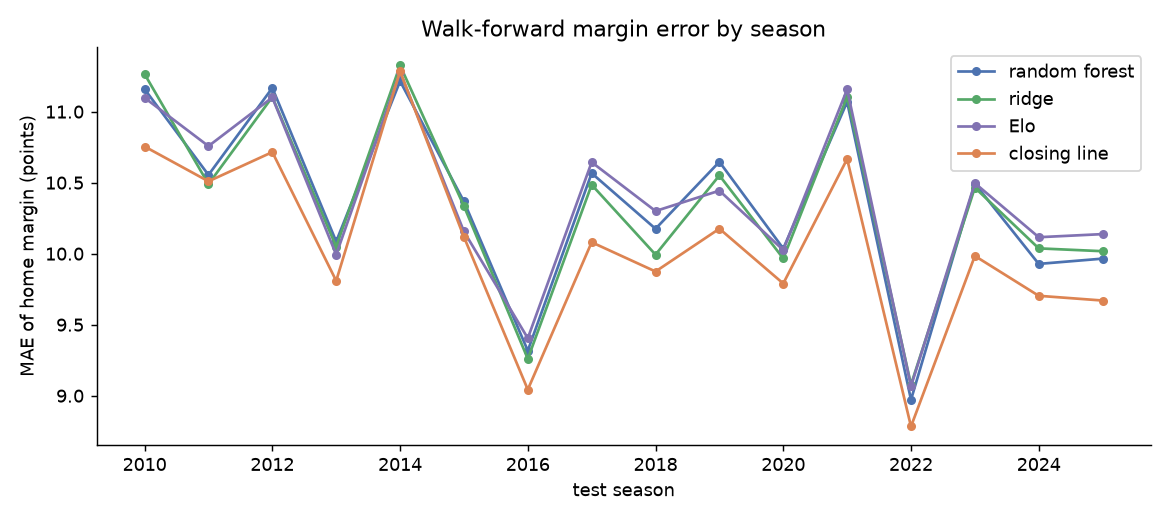
\includegraphics[width=0.95\textwidth]{rf_mae_by_season.png}
\caption{Margin error by test season. All methods share the hard and easy seasons; the closing line is lowest in 15 of 16.}
\label{fig:mae_season}
\end{figure}

\begin{figure}[H]
\centering
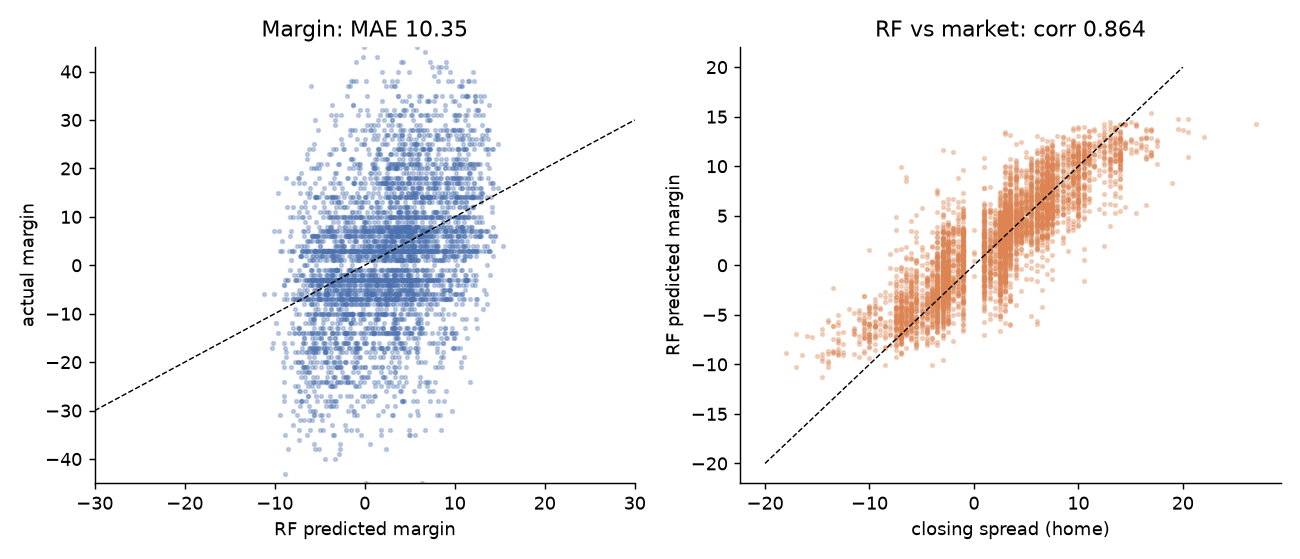
\includegraphics[width=0.95\textwidth]{rf_pred_vs_actual.png}
\caption{Left: predicted against actual margin. Right: the forest's margin against the closing spread (correlation 0.86).}
\label{fig:pred_actual}
\end{figure}

\subsection{The two-output structure}

Because the forest predicts a point in the $(h,a)$ plane, its residuals describe a two-dimensional distribution around that point (Table~\ref{tab:bivariate}, Figure~\ref{fig:bivariate}). The correlation between the home and away residuals is 0.01: once the two means are set, the leftover error in one score says nothing about the other. Residual spread grows with the predicted score, so high-scoring games are less predictable in points, as a Poisson-like scoring process implies. Calibration per score is good: when the forest predicts 20 points the team scores 20 on average, across the range 15 to 33.

\begin{table}[H]
\centering
\small
\begin{tabular}{lcc}
\toprule
\textbf{Quantity} & \textbf{Home} & \textbf{Away} \\
\midrule
Standard deviation of the actual score & 10.21 & 9.83 \\
Standard deviation of the residual & 9.64 & 9.36 \\
Range of predicted scores & 15.8 to 33.3 & 13.3 to 30.4 \\
Residual s.d., lowest third of predictions & 9.20 & 8.88 \\
Residual s.d., highest third of predictions & 10.11 & 9.76 \\
\bottomrule
\end{tabular}
\caption{Residual structure of the two-output forest, 4,363 out-of-sample games. Residual correlation 0.011.}
\label{tab:bivariate}
\end{table}

\begin{figure}[H]
\centering
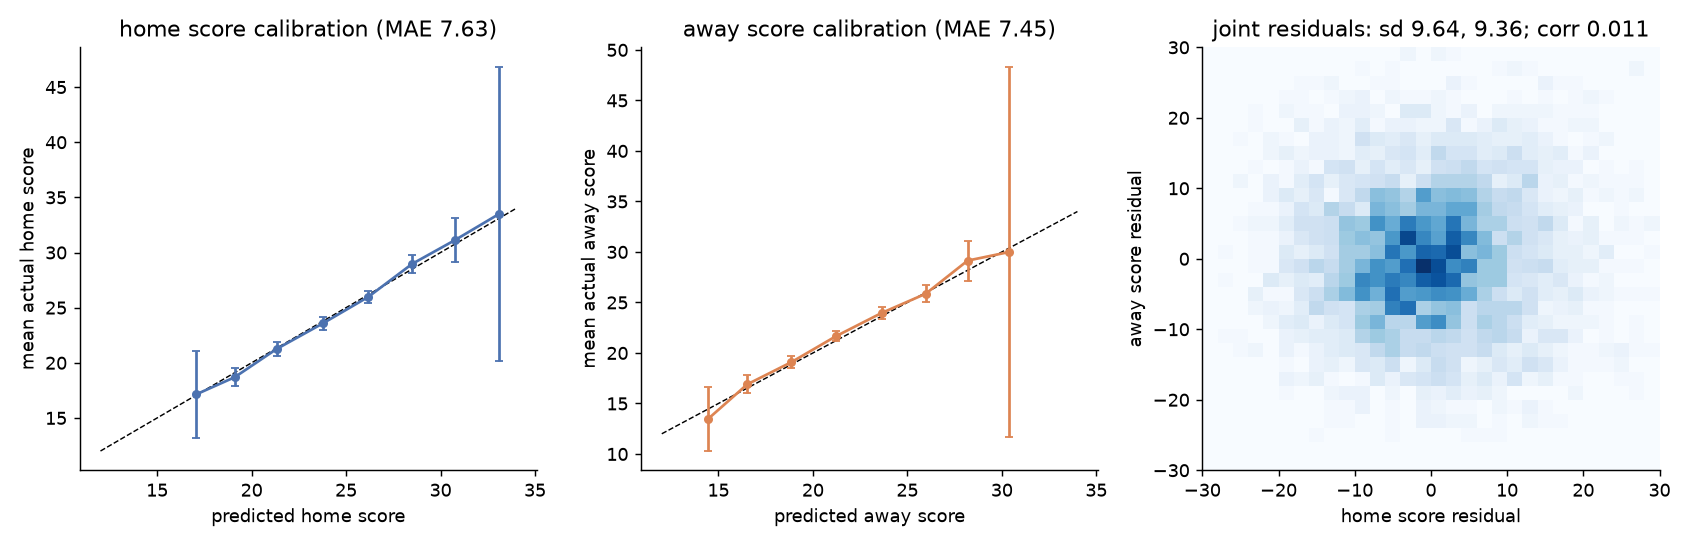
\includegraphics[width=0.98\textwidth]{rf_bivariate.png}
\caption{Calibration of the home and away score predictions and the joint distribution of the two residuals.}
\label{fig:bivariate}
\end{figure}

These residual statistics are the parameters $(\sigma_h,\sigma_a,\rho)$ of the probabilistic extension suggested by Professor Amine. Used as a pooled bivariate normal around the two predicted scores, they give a home-win probability with Brier score 0.2207 over 2016--2025, against 0.2220 for Elo and 0.2108 for the de-vigged moneyline; placing the two predicted means on the empirical grid of Section~\ref{sec:pricing} gives 0.2213. The probabilities are calibrated (Figure~\ref{fig:rf_cal}); the gap to the market is in sharpness, not bias.

\begin{figure}[H]
\centering
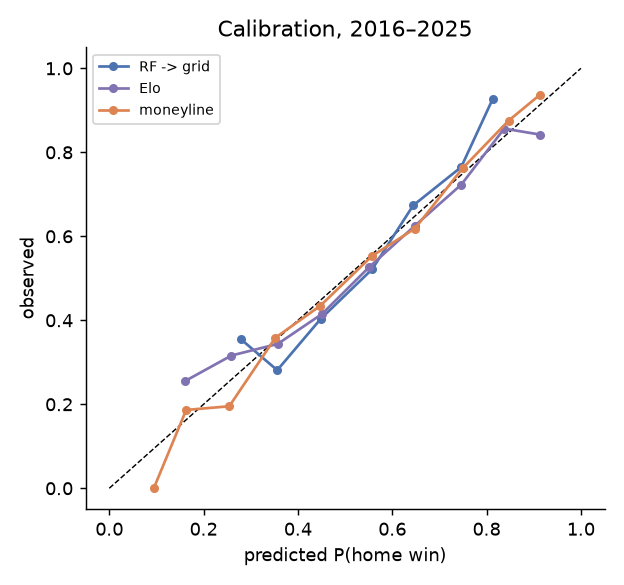
\includegraphics[width=0.5\textwidth]{rf_calibration.png}
\caption{Calibration of home-win probabilities, 2016--2025.}
\label{fig:rf_cal}
\end{figure}

\subsection{What the forest uses}

Averaged over the sixteen fits, the five most important features are all team-strength summaries from results: the difference in opponent-adjusted weighted margin, the difference in weighted margin, and the three Elo features (Figure~\ref{fig:importance}). The first play-by-play feature is yards per play, followed by the starting quarterback's success rate and EPA per dropback and points per drive. Injury, rest and weather features are far down the list. Most of what the model knows is how good each team has been; the efficiency and quarterback features refine that at the margin. The forest used all 759 features with no selection or tuning and matched a regularised linear model, which is what Professor Shasha expected.

\begin{figure}[H]
\centering
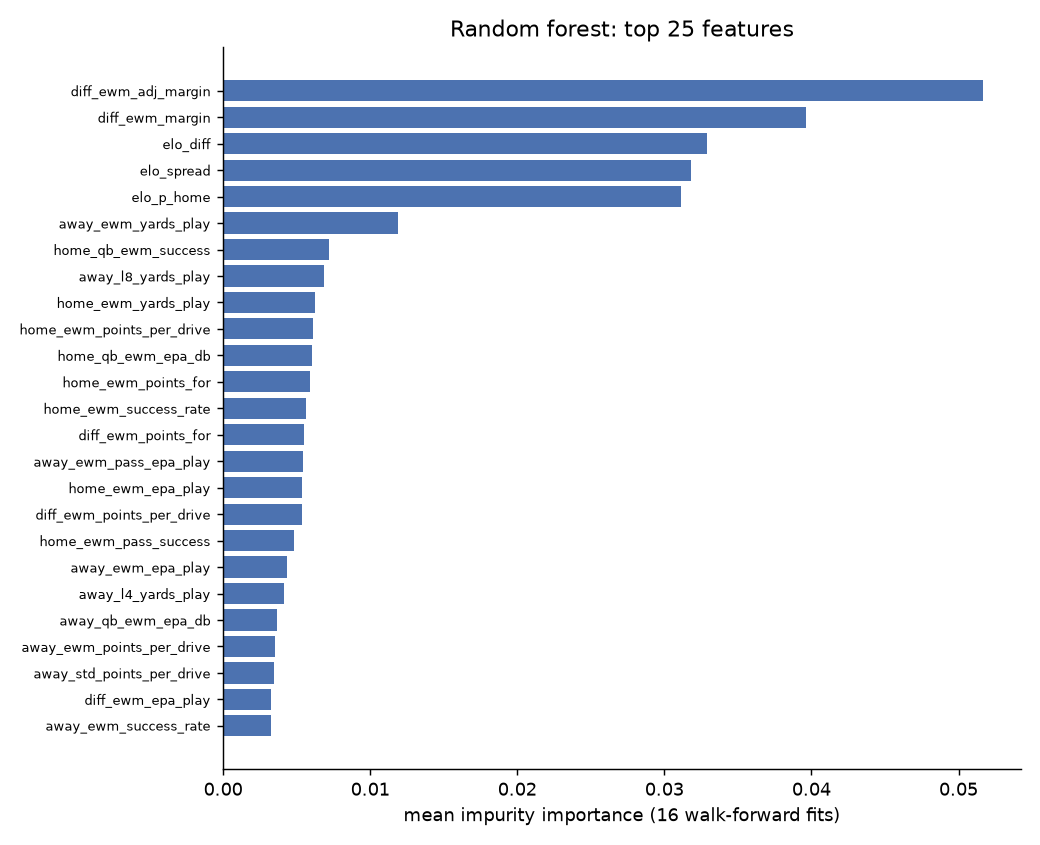
\includegraphics[width=0.75\textwidth]{rf_importance.png}
\caption{Top 25 features by mean impurity importance over the sixteen walk-forward fits.}
\label{fig:importance}
\end{figure}

\subsection{Can an ensemble do better?}

Professor Shasha asked whether an ensemble of the models we have, or can obtain, improves on them. We stacked by least squares, fitting weights on earlier seasons' out-of-sample predictions and applying them to the next season, 2013--2025. To our three models we added two public forecasts, nfelo~\cite{nfelo} (a public Elo variant with a quarterback adjustment; we use its rating difference before any regression toward the market) and FiveThirtyEight's Elo (available to 2020), and the sportsbook \emph{opening} line, which the nfelo files carry (Table~\ref{tab:ensemble}, Figure~\ref{fig:ensemble}).

\begin{table}[H]
\centering
\small
\begin{tabular}{lcp{6cm}}
\toprule
\textbf{Forecast} & \textbf{Margin MAE} & \textbf{Note} \\
\midrule
Random forest (ours) & 10.22 & \\
Ridge (ours) & 10.20 & \\
Elo (ours) & 10.25 & \\
Stack of our three & 10.18 & weights 0.19 / 0.36 / 0.51 \\
nfelo, pure model & 10.01 & history back-computed with the current model, so optimistic \\
Stack: ours + nfelo & 10.04 & our models receive weight near 0 \\
Opening line & 10.02 & \\
Closing line & 9.92 & \\
Stack: ours + nfelo + closing line & 9.95 & closing line 0.58, nfelo 0.72, ours near 0 \\
\bottomrule
\end{tabular}
\caption{Stacking test, home margin, 2013--2025 (3,562 games with all forecasts available).}
\label{tab:ensemble}
\end{table}

\begin{figure}[H]
\centering
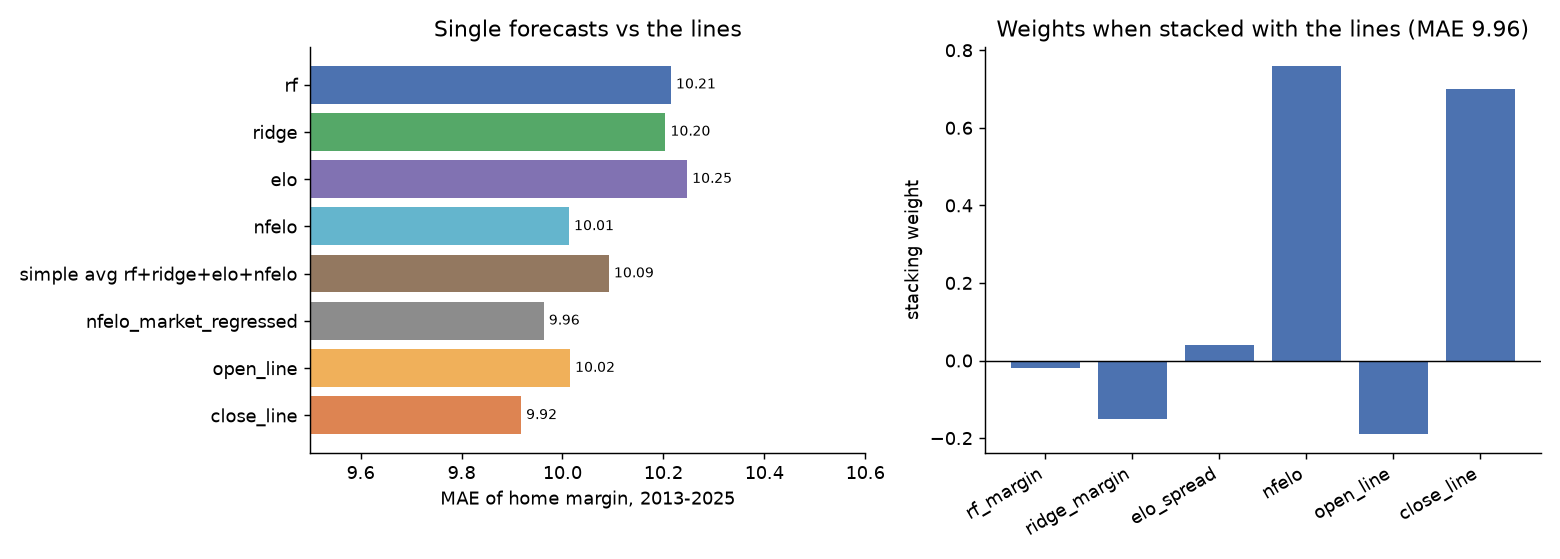
\includegraphics[width=0.98\textwidth]{ensemble_external.png}
\caption{Left: single forecasts and the lines. Right: stacking weights when our models, nfelo and both lines are combined.}
\label{fig:ensemble}
\end{figure}

Averaging our own models gains only a few hundredths of a point, because their predictions are correlated at 0.89--0.94. nfelo is a better single forecast than anything we built, by about 0.2 points, which we attribute to its quarterback adjustment and to its published history being generated by the current version of the model. Most important, no stack improves on the closing line: whenever the line is a component it takes nearly all the weight. The same holds for totals, where the opening total (10.47) is in fact slightly better than the closing total (10.53) in this sample. Ensembling what we have does not beat the market; an ensemble that could would need forecasts carrying information the market does not yet have.

\subsection{Full distributions and the Vegas lines}

The second question was whether the models can give a distribution for the margin and the total and how it compares with the lines. The two predicted scores set the centre, and the distribution around them comes either from the bivariate normal with the residual covariance or from the empirical grid tilted so that its mean margin and total match the forest (Figure~\ref{fig:gamedist}). From either, the probability of any outcome is a sum: $P(\text{home wins})$, $P(\text{home covers the spread})$, $P(\text{over the total})$.

\begin{figure}[H]
\centering
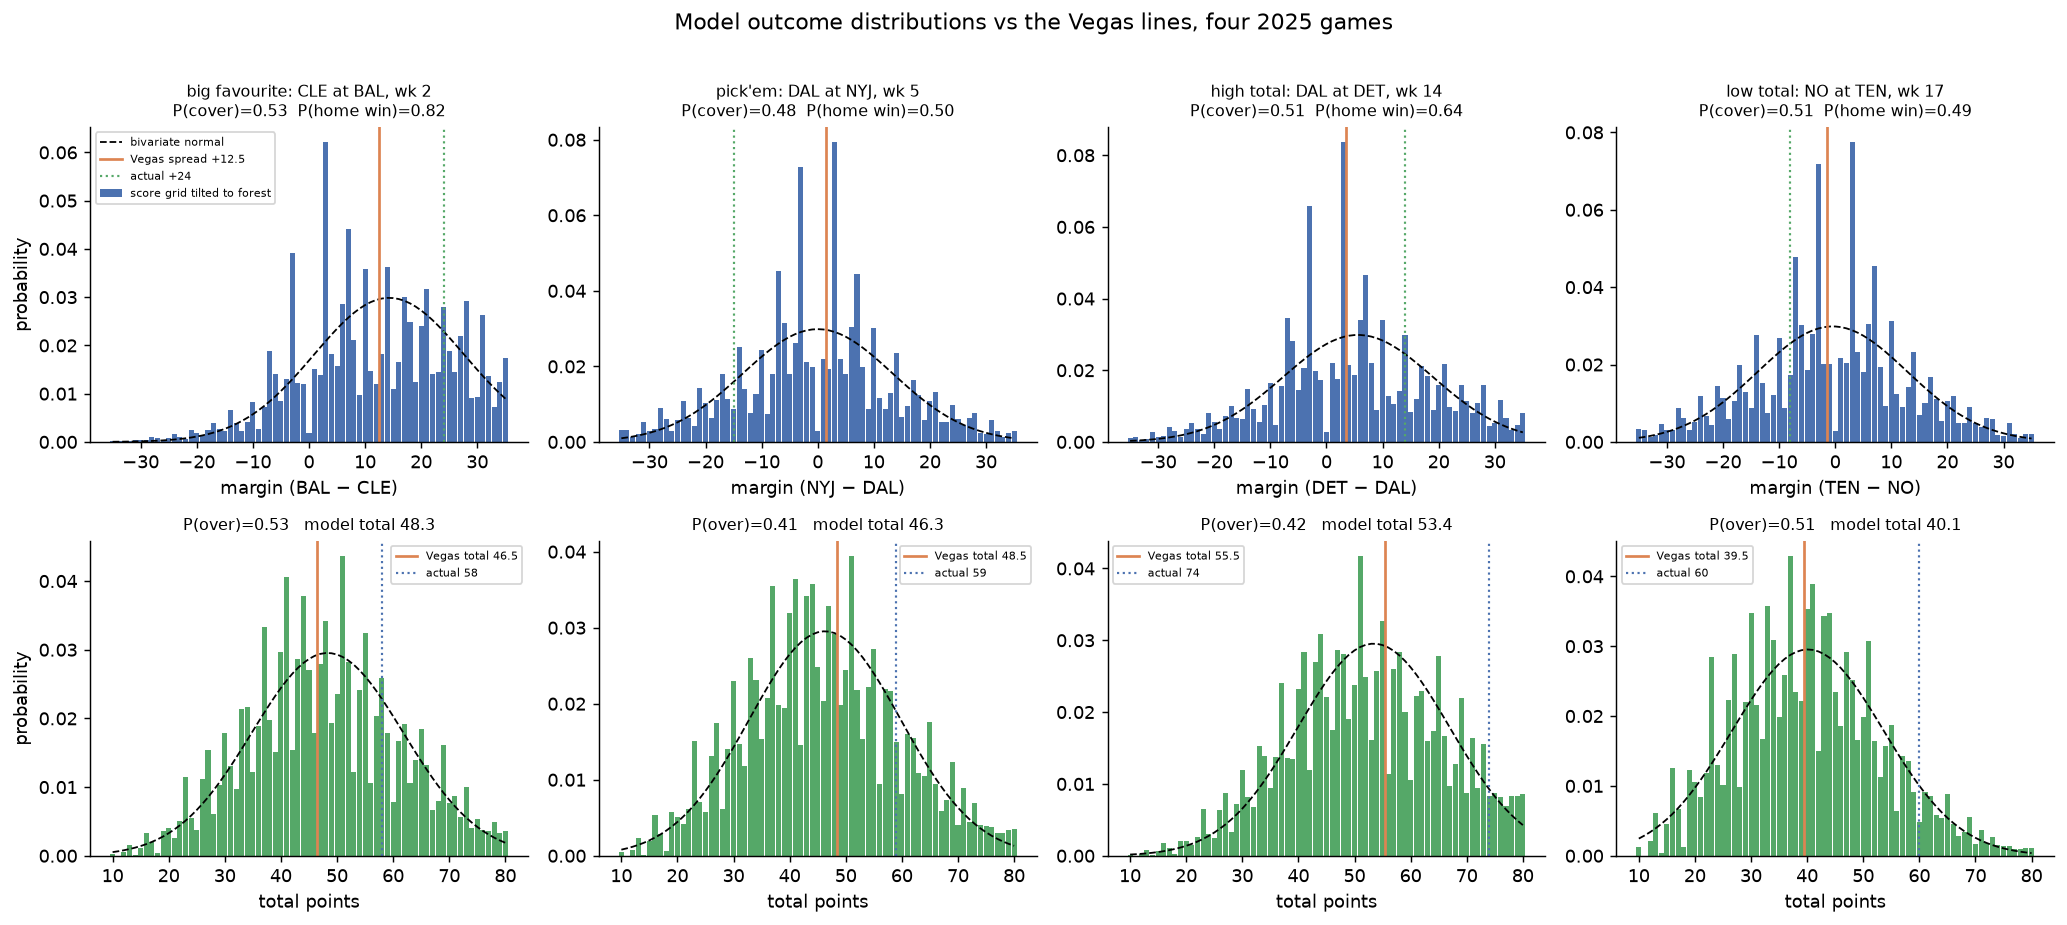
\includegraphics[width=\textwidth]{game_distributions.png}
\caption{Four 2025 games. Top: margin distribution from the tilted score grid (bars) and the bivariate normal (dashed), with the Vegas spread (orange) and the actual margin (dotted). Bottom: the same for the total.}
\label{fig:gamedist}
\end{figure}

Across all 2,758 games from 2016 to 2025, the model's $P(\text{cover})$ averages 0.50 with a standard deviation of 0.09 and $P(\text{over})$ averages 0.49 with a standard deviation of 0.08; only a quarter of games get a cover probability outside 0.40--0.60. The calibration of these probabilities against outcomes is flat (Figure~\ref{fig:coverover}): when the model says 65\% to cover, teams cover about 52\%. Brier scores of 0.257 for cover and 0.255 for over, against 0.25 for a coin, say the same thing. The distributions are internally consistent and calibrated for outcomes the market has not priced, but they do not know which side of the Vegas number will hit. This is the expected result for an efficient line, and it is the reason the engine's value lies in pricing the whole distribution consistently rather than in picking sides.

\begin{figure}[H]
\centering
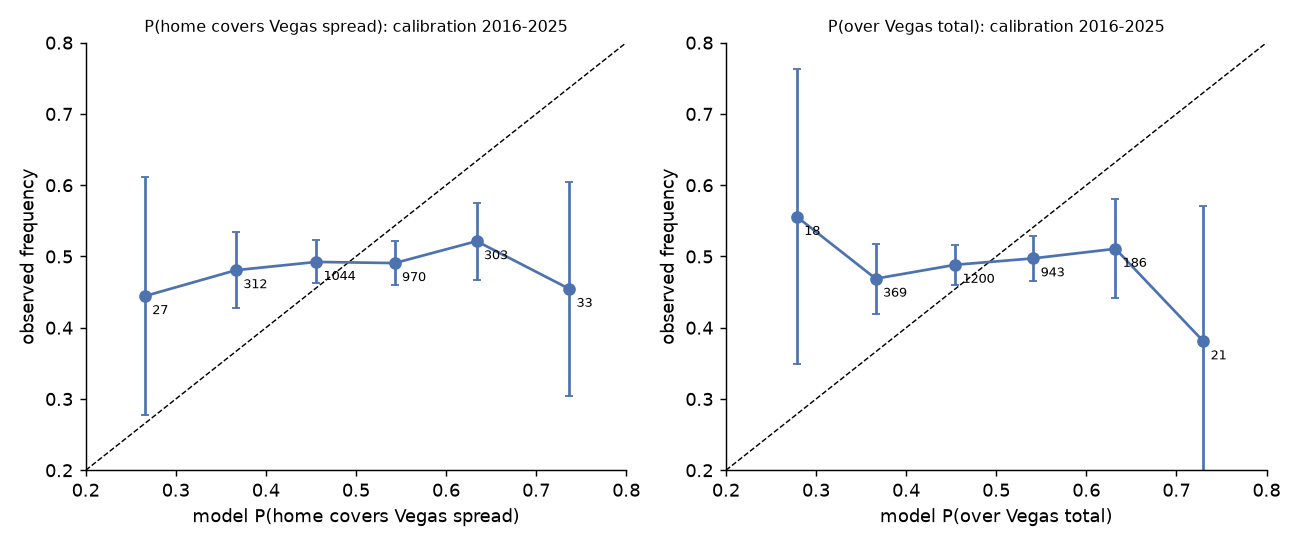
\includegraphics[width=0.95\textwidth]{cover_over_calibration.png}
\caption{Calibration of the model's cover and over probabilities, 2016--2025; bin sizes shown.}
\label{fig:coverover}
\end{figure}

\section{Conclusions and Next Steps}

\subsection{What we have learned}
\begin{enumerate}[nosep]
\item For a binary contract, price, probability and the profit-and-loss distribution are the same thing; for a portfolio on one game, a joint distribution over the final score is the risk model. VaR and expected shortfall are then exact sums, with no covariance matrix or simulation.
\item The NFL score distribution is discrete in ways that matter for pricing: 3-point margins are 2.9 times as likely as a normal model says, and margin and total always share parity. An empirical score grid, repositioned by exponential tilting, prices a game's whole ladder of contracts to within a cent of the Kalshi order book once the dispersion is calibrated.
\item Point accuracy is capped near the Vegas closing line. Our two-output random forest, a linear model, Elo, a public Elo variant and every stack of them sit 0.1 to 0.4 points behind the line, as the literature has found since 1980. The forest and the linear model tie, so with 7,000 games the information is in the features, and the features are mostly ratings.
\item The forest's two score predictions are calibrated, and their residuals are uncorrelated with standard deviations near 9.5 points that rise with the level of scoring. Those are the parameters needed to turn two predicted scores into a probability for any outcome.
\item The resulting cover and over probabilities are calibrated for outcomes the market has not priced but carry no information about which side of the Vegas number will hit. The engine's value is in pricing the whole distribution consistently, not in picking sides against the market.
\item Leakage is the dominant risk in this kind of work and is easy to introduce from a well-maintained public dataset. A perturbation test and a sanity check against the literature's error levels are both needed.
\end{enumerate}

\subsection{Next steps}
\begin{enumerate}[nosep]
\item \textbf{Probabilistic head.} A model that predicts $(\mu_h,\mu_a,\sigma_h,\sigma_a,\rho)$ per game, trained on the bivariate negative log-likelihood, and used to position and scale the empirical grid. The toy example shows a dispersion parameter removes the remaining tail error.
\item \textbf{Remaining suggested methods} on the same feature table: LARS for a sparse linear model, gradient boosting, PCA and UMAP as exploration, and a cascade-correlation network as a final comparison.
\item \textbf{Offence and defence ratings} in the Glickman and Stern~\cite{glickmanstern1998} state-space form, so each predicted score has its own strength input rather than a single Elo; recency weighting for the scoring environment; a stadium lookup for travel distance.
\item \textbf{Risk layer.} Represent a book of Kalshi positions as a payoff vector on the score grid; compute ES, worst cell and probability of loss exactly; measure in-play jump risk from the trade tape, where hourly price changes are 17 cents against 1 cent pre-game; add the quoted-spread curve (which scales with $p(1-p)$, not with strike distance) as the liquidation cost.
\item \textbf{Live record.} Update weekly through the 2026 season: new games, new Kalshi prices, re-run the walk-forward, accumulate out-of-sample forecasts against the market.
\end{enumerate}

\subsection{Research log}
\begin{description}[nosep,leftmargin=0pt,labelindent=0pt]
\item[30 September 2026] Framed pricing as outcome modelling; surveyed the sports-pricing literature; pulled Kalshi markets, trades and candlesticks and nflverse results; exploratory analysis of the score distribution and of Kalshi liquidity; worked example of the tilted empirical grid against a live order book.
\item[7 October 2026] Literature survey of NFL prediction and market efficiency; catalogue of data used in the literature against what nflverse provides; built the 805-column feature table with the leakage test; first two-output random forest, walk-forward results, bivariate residual structure.
\item[21 October 2026] Follow-ups from Professor Shasha: ensemble and stacking test with public forecasts and the opening line; full margin and total distributions compared with the Vegas lines; cover and over calibration.
\end{description}


\vspace{6pt}
\authorcontributions{Conceptualization: D.S. and S.K.P.; methodology, software, data curation, analysis and writing: S.K.P.; supervision and review: D.S.}
\funding{This research received no external funding.}
\dataavailability{Data are from the public nflverse project and the Kalshi API; code is in the project repository.}
\conflictsofinterest{The authors declare no conflict of interest.}

\reftitle{References}
\bibliography{riskpredictor}

\PublishersNote{}
\end{document}
